% Extracted from attraction_wfigs.docx; see PLAN.md and tools/extract_pilot.py.

% DOCX paragraph 110
\chapter{The Fathers of Gravity}\label{ch:02}

% DOCX paragraph 113
To fully understand gravity, it may be helpful to take a small step back in time and
adopt a historical perspective rather than a physical one. This interlude will be rather
short and limited to those scientists who, more than others, have contributed to shaping
our understanding of the subject.

% DOCX paragraph 116
\section{Galileo Galilei: The Importance of the Method}\label{sec:02-galileo}

% DOCX paragraph 118
Let us start from the beginning. To paint a historical portrait of the theory of
gravity, and thus acknowledge those who its ``fathers'' were, we cannot help but start
in Italy, in particular in Pisa. There, between the end of the sixteenth century and the
beginning of the seventeenth century, Galileo Galilei\index{Galilei, Galileo}
(1564-1642) was the first to try to decode the dynamics (that is, the state of rest or
motion) of physical objects. These were still difficult times for science: deductive
logic and experimental pragmatism inevitably succumbed to philosophical and religious
dogmatism. Galileo experienced this first-hand when the accusation of heresy was
levelled at him in 1633.

% DOCX paragraph 119
Nonetheless, adopting \emph{the scientific method} that he himself had introduced,
Galileo\index{Galileo!scientific method}\index{scientific method} intended to study
quantities, such as the velocity and the state of motion at constant velocity. In this
way, he empirically derived the so-called \emph{principle
of}\index{principle of!inertia} \emph{inertia}, which, thanks to Isaac
Newton\index{Newton!Isaac}, became an axiom of dynamics more than a century later.

% DOCX paragraph 121
This principle states that, in the absence of external forces, a body maintains its
state of uniform rectilinear motion (i.e., it continues to move at a constant speed
along a straight trajectory) and remains at rest if it is initially at rest. The meaning
of this principle is less detached from reality than it may seem; we experience its
effects every time we are on a bus or the subway and the vehicle starts or brakes. In
the first case, we are accelerated in the opposite direction to that of travel simply
because we tend to maintain a state of rest. In the second case, however, we are
accelerated in the direction of travel since our ``inertia'' compels us to maintain the
state of motion we had before. Thus, we continue to move forward.

% DOCX paragraph 122
This discovery led Galileo to formulate the \emph{Galilean principle
of}\index{principle of!relativity} \emph{relativity,} from which the so-called
\emph{Galilean transformations}\index{Galileo!transformations} \emph{between two
reference systems} follows. In essence, it states that the laws of physics are the same
in two frames of reference (or, equivalently, for two observers) that are moving at
constant or zero speed. As we will see, this principle was also useful to Einstein about
three centuries later, and that is why Galileo can be considered the ``first
relativist''.

% DOCX paragraph 123
However, besides objects in uniform motion, Galileo was also very interested in objects
subject to forces and, therefore, experiencing acceleration. The simplest way to study
objects in accelerated motion is to let them fall, for reasons that will soon become
clear. Therefore, Galileo spent most of his time on top of towers (like the one in Pisa,
and those in Bologna and Florence), concentrating his attention on the motion of
``gravi''\index{gravi (Galileo Galilei)} (from the Latin ``gravis'', or heavy), i.e., of
heavy objects in free fall\index{free fall}.

% DOCX paragraph 124
A practical problem that Galileo faced in his experiments was the fairly high
gravitational acceleration of physical objects and, although he exploited relatively
tall buildings, the time taken by those objects to reach the ground was still very short
and, therefore, difficult to measure. He then resorted to a device that allowed him to
slow down the fall time as he pleased: the so-called \emph{inclined plane}. This is a
right-angled triangle with the hypotenuse facing upwards; by varying the \emph{attack
angle} (i.e., the acute angle), it is possible to vary the component of the ``force'' of
gravity \index{gravitational!force}involved in the motion. By exploiting this simple but
ingenious solution, Galileo was able to slow down the motion of heavy spheres rolling
down a plane that he had carefully polished to reduce friction. In this way, he was able
to perform very accurate measurements.

% DOCX paragraph 125
In this way --- and as explained in his most important work, the \emph{Dialogue
Concerning the Two Chief World Systems}, published in 1632 --- Galileo calculated that
the gravitational acceleration (that is, the acceleration of a body subject to the
action of gravity) was equal to about 9.80 metres per square second
(m/s\textsuperscript{2}). This estimate is essentially correct, which is quite
surprising if one thinks of early seventeenth-century technology and the precision it
allowed. Today, we know that this acceleration varies according to the position on the
surface of the Earth, with values ranging between 9.764 m/s\textsuperscript{2} and 9.834
m/s\textsuperscript{2}, and changes in relation to altitude. However, the standard
reference value of 9.80665 m/s\textsuperscript{2} is still very close to Galileo's
measurement. Furthermore, Galileo estimated that the distance travelled by a
free-falling object increases with the square of the time taken to fall --- a result we
now know to be correct.

% DOCX paragraph 126
To this day, historians still wonder whether Galileo really did conduct experiments such
as dropping objects of different material (wood, gold, and silver), or of the same
material but with different masses (cannonballs and musket balls), from the top of the
Tower of Pisa. One thing is certain, however: in his \emph{Dialogue} he summarised a
series of considerations (both his own and those of previous scientists) pointing to the
evidence of a universal law of gravitation. This hypothesis, which Galileo never
formulated in explicit terms as a law, essentially states that all objects in a
gravitational field accelerate in the same way, regardless of their mass or composition.
In other words, Galileo had already guessed that if you throw a cannonball and a musket
ball from a high tower, they will reach the ground simultaneously.

% DOCX paragraph 127
The importance and depth of this hypothesis --- which today we call \emph{Equivalence}
\emph{Principle}\index{equivalence principle}\index{principle of!equivalence} and know
to be correct with a relative accuracy of one-millionth of a billion --- is particularly
valuable for two distinct reasons. The first is that it openly clashed with Aristotle's
assertion, namely, that gravitational acceleration is directly proportional to the
weight of an object, so that heavy ones should fall faster than light ones. It is
difficult for us, with our modern scientific mindset, to imagine the intellectual effort
and courage needed to take sides against the cultural authority represented by the
Aristotelian dogmatic principle at the beginning of the seventeenth century. The second
is that to believe (contrary to our direct experience) a cannonball and a feather in
free fall\index{free fall} accelerate in the same way required a considerable leap of
imagination. Indeed, Galileo's conclusion is far more revealing than it may appear and
points to a consideration of fundamental importance: the evidence gained through our
daily experience can be misleading! More specifically, the reason for which, in our
everyday experience, the feather reaches the ground after the cannonball is not because
the feather experiences a smaller gravitational acceleration but because it is subject
to proportionally larger friction than the cannonball. If dropped from a tower in a
vacuum\index{vacuum} (therefore, in the absence of drag), the feather and the cannonball
would touch the ground simultaneously (this was indeed demonstrated at the end of the
last Apollo 15 moon walk and can be watched on public archival videos). Obviously,
Galileo could not create vacuum conditions in his experiments from the Tower of Pisa,
but his imagination was powerful enough to show him the underlying truth. In the
following pages, we will see that a similar feat of imagination will be made by Einstein
almost three hundred years later.

% DOCX paragraph 128
Galileo's results and, above all, the first use of a scientific
method\index{scientific method} (\emph{his} very own method!) to abandon a metaphysical
interpretation of reality in favour of a deductive experimental approach were
undoubtedly essential for what was discovered and understood about gravity after him.
However, at the time of his death in 1642, knowledge on the subject did not stray far
from pure empirical evidence. It took about 40 years for a new and more complete view of
gravitational interaction to emerge.

% DOCX paragraph 131
\section{Isaac Newton: A Complete Mathematical Picture}\label{sec:02-newton}

% DOCX paragraph 133
The first mathematical formulation of the theory of gravitation is indisputably
associated with Isaac Newton (1642-1726), who consequently may rightly be counted among
the fathers of gravity. There is little doubt that the contributions of this brilliant
mind to the construction of modern science have been enormous and wide-ranging: from
astronomy to mathematics; from theology to alchemy \ldots{} to illustrate them, if only
briefly, I would need to write another book. But that\textquotesingle s not my aim here.
What I want to focus on, instead, is Newton\textquotesingle s contributions to the
understanding of gravity contained in what is considered his main work: \emph{The
Mathematical Principles of Natural Philosophy} or, more simply, the
\emph{Principia}\index{Principia Mathematica} (from the original Latin title:
\emph{Philosophiae Naturalis Principia Mathematica}).\index{Newton!Principia}

% DOCX paragraph 134
In this three-volume treatise, published in 1687, Newton introduced three principles of
the dynamics of bodies that represent the backbone of the so-called Newtonian physics.
Although well-known and almost emblematic of our scholastic knowledge of physics, it is
helpful to recall them briefly:

\begin{enumerate}
\def\labelenumi{\arabic{enumi}.}
\item

  % DOCX paragraph 136
  \emph{Principle}\index{principle of!inertia} \emph{of inertia}: in the absence of
  forces, a body will maintain its state of rest or uniform rectilinear motion.
\item

  % DOCX paragraph 137
  \emph{Principle of conservation of momentum}
  \index{principle of!conservation of momentum} (given by the product of mass and
  velocity): in the presence of a force, the change in motion (i.e., the acceleration)
  is proportional to the resulting force applied and occurs along the direction in which
  the force is exerted.
\item

  % DOCX paragraph 138
  \emph{Principle of action and reaction}\index{principle of!action and reaction}: for
  every action of one body upon another, there is a corresponding equal and opposite
  reaction.
\end{enumerate}

% DOCX paragraph 140
Alongside these three principles (and taking gravity as belonging to a particular class
of forces), Newton also proposed the so-called \emph{universal law of gravitation})
\index{Newton!universal law of gravitation}. \index{gravitational!force}The basic
properties of the force of gravity postulated by Newton can then be summarised as
follows:

\begin{enumerate}
\def\labelenumi{\arabic{enumi}.}
\item

  % DOCX paragraph 142
  \emph{It is an attractive force between two massive bodies.} In other words, this
  force manifests itself as an attraction between two bodies with mass (i.e., a property
  that can be associated with any material physical body) along the direction that joins
  them.
\item

  % DOCX paragraph 143
  \emph{It is an instant force.} In other words, the two bodies experience this force
  immediately so that if something changes in one of the two (the mass or the position,
  for example), the other body ``knows'' about it instantly.
\item

  % DOCX paragraph 144
  \emph{It is a force proportional to the masses of the two bodies involved.} Hence, the
  greater the mass of the bodies, the greater the intensity of the force. Note that this
  force does not depend on the composition of the bodies themselves or on their size.
  The only thing that matters is how massive they are. A direct consequence of this
  property is that a body without a mass is not subject to a gravitational force.
\item

  % DOCX paragraph 145
  \emph{It is a force inversely proportional to the square of the distance between the
  two bodies.} Stated differently, once the mass is fixed, bodies at a great distance
  attract much less than bodies that are close to each other. It follows that bodies at
  an infinite distance do not attract each other at all; similarly, the same body would
  experience a gradually weaker force as it moves away from a centre of gravitational
  attraction.
\end{enumerate}

% DOCX paragraph 147
When writing this book, I made a deliberate choice to limit mathematics to the bare
minimum but not to do without. When used at the right moment, mathematics can help us
understand the laws of physics, even when used only descriptively. In this spirit, we
can use mathematical expressions --- the same ones Newton used over three centuries ago
--- to summarise what is expressed in the four points above. In essence, those four
statements can be condensed into this "conceptual equation":

% DOCX paragraph 153
\[\begin{pmatrix}
strength\ of\ the \\
force\ of\ gravity
\end{pmatrix} = \frac{(mass\ of\ object\ 1)\  \times \ (mass\ of\ object\ 2)}{(distance\ between\ object\ 1\ and\ 2)^{2}}\]

% DOCX paragraph 155
The most important aspect of the expression above (which should be readable even for
those who are ``allergic'' to mathematics) is the ``equals'' sign. Indeed, the
\textbf{=} symbol, which we are all familiar with, makes the above expression an
\emph{equation}, thus establishing that what appears on its left-hand side is equivalent
to what is written on its right-hand side. However, if we wanted to translate all this
into an actual mathematical equation, then the universal law of gravitation would be
expressed by the equation:

% DOCX paragraph 157
\begin{equation}\label{eq:02-01}
{\overrightarrow{F}}_{grav} = \  - \ G\frac{M_{1}M_{2}}{r^{2}}\left( \frac{\overrightarrow{r}}{r} \right)
\end{equation}

% DOCX paragraph 159
Here, \emph{M}\textsubscript{1} and \emph{M}\textsubscript{2} are the masses of the two
bodies, while \emph{r} is their distance. The small arrows above
\({\overrightarrow{F}}_{grav}\) and \(\overrightarrow{r}\) remind us that they express
quantities with a strength and a direction. These are also called \emph{vectors}: the
vector\index{vector} of the gravitational force\index{gravitational!force} and the
vector of the distance between the two bodies,
respectively.\textsuperscript{\hyperlink{note:02-01}{1}} Finally, the symbol \emph{G}
simply represents a constant of proportionality between what is written on the right and
what appears on the left; it has no deep physical meaning and must be determined through
experiments. Today, we know that, according to the International System of units,
\emph{G} = 6.67408 x 10\textsuperscript{--11} m\textsuperscript{3}/(kg
s\textsuperscript{2}).

% DOCX paragraph 160
The striking and fascinating aspect of the simple Equation \eqref{eq:02-01} is that, with it,
Newton was able to provide a satisfactory and extremely accurate description of
gravitation. Thanks to this mathematical tool, it was possible to interpret any
phenomenon that had something to do with gravity: to explain why an apple falls from a
tree or why the Earth orbits the Sun. Combined with the ideas put forward by the Polish
astronomer Nicolaus Copernicus\index{Copernicus, Nicolaus} (1473-1543) (namely, that all
the planets close to us revolve around the Sun) and the German astronomer Johannes
Kepler\index{Kepler} (1571-1630) (that orbital\index{orbit} motion occurs along
elliptical trajectories with the Sun positioned in one of the two foci),
Newton\textquotesingle s universal law of gravitation \eqref{eq:02-01} could explain all the
astronomical observations of his time. By virtue of this, and for about two centuries,
it was possible to make extremely accurate predictions about the motion of the celestial
objects in our solar system.

% DOCX paragraph 161
Another remarkable property of Newton's expression is that it is ``universal''; in other
words, it is all we need to explain, at least approximately, \emph{any} gravitational
phenomenon on Earth. Whether we want to build the longest bridge or the tallest
skyscraper, we need nothing more than this simple and beautiful Equation \eqref{eq:02-01}.
Nonetheless, such an equation and the concepts on which it is built are
\emph{incorrect}. More specifically, we are now aware that:

\begin{enumerate}
\def\labelenumi{\arabic{enumi}.}
\item

  % DOCX paragraph 163
  \emph{Gravity is not a force.} The concept of ``gravitational force'' is not only not
  useful but also misleading. Therefore, it should be replaced by another concept,
  better suited to explain the nature of gravity, however more complex to express
  mathematically, and therefore farther from our intuitive understanding of nature.
\item

  % DOCX paragraph 164
  \emph{Gravity is not instantaneous}\index{interaction!instantaneous}\emph{.} Modern
  physics is built on the opposite assumption: every physical interaction propagates
  with a finite speed, the fastest of which is the speed of light. Gravity too is
  subject to this restriction, so a change in the gravitational field has to propagate
  over a finite time before it is detected.
\item

  % DOCX paragraph 165
  \emph{The mass alone is not enough to describe gravity.} In addition to the magnitude
  of the mass, its distribution in space must be considered. In other words, it is
  necessary to know the length-scale over which the mass is contained. In the case of an
  extended object such as the Sun, the properties of gravity relate as much to its mass
  as to its radius.
\end{enumerate}

% DOCX paragraph 167
For over two centuries, Newton\textquotesingle s law of gravitation was used
extensively, and its undisputed validity was confirmed by an endless series of
experimental successes, thus making it, among other things, the pillar of navigation
and, therefore, of maritime trade. However, a simple astronomical observation was
sufficient to undermine a theory that until then seemed written in the stone of
universal laws and was treated with an almost reverential attitude.

% DOCX paragraph 168
A small crack opened up in the noble and imposing facade of the building Newton had
erected, conjuring up its inevitable collapse: \emph{the precession of the
perihelion}\index{perihelion} of Mercury. This seemingly enigmatic name refers to a very
easily observable sequence of events. Every 88 days or so, Mercury makes a complete
orbit\index{orbit} around the Sun, reaching the point in the orbit when it is closest to
the star, that is, the \emph{perihelion}. In Newton\textquotesingle s theory, this point
is always the same, fixed and invariable unless external factors intervene. In essence,
Mercury\textquotesingle s orbit around the Sun must be ``closed'', that is, it must
return to exactly the same point after an orbital period. This is shown in Figure \ref{fig:02-01},
where the dashed ellipse indicates Mercury's orbit according to Newton\textquotesingle s
law of gravity.

% DOCX paragraph 170
\begin{figure}[htbp]
\centering
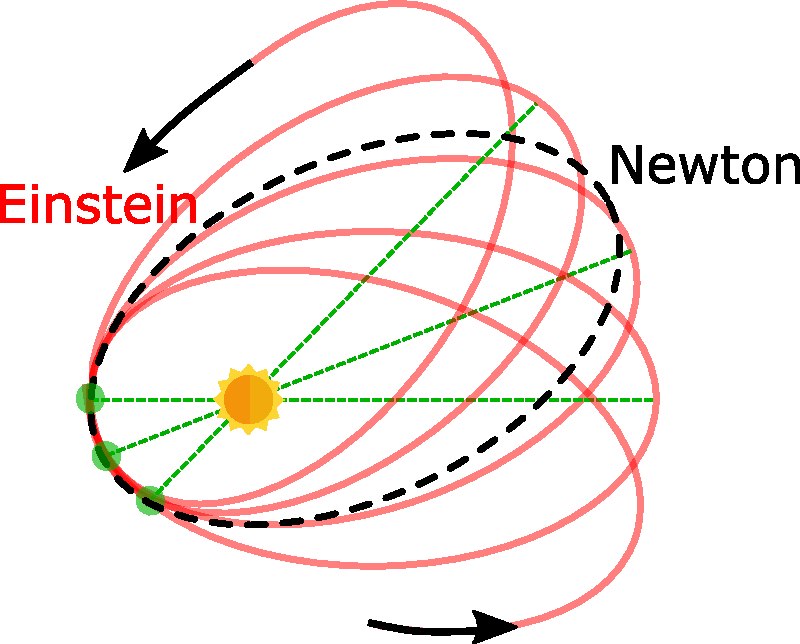
\includegraphics[width=0.82\linewidth]{../figs/pdf/en/fig-02-01.pdf}

% DOCX paragraph 173
\caption{\emph{Schematic illustration of Mercury\textquotesingle s orbit. According to
Newton\textquotesingle s theory of gravitation, it should be closed (dashed ellipse),
while Einstein\textquotesingle s theory of gravity (solid line) tells us that it must
continuously change, with the perihelion}\index{perihelion} \emph{moving at each orbital
period.}}\label{fig:02-01}
\end{figure}

% DOCX paragraph 175
However, astronomical observations tell us something entirely different! Even after
considering the orbital variations due to other bodies in the solar system,
Mercury\textquotesingle s perihelion\index{perihelion} changes more than Newton
predicted, i.e., by 0.1035 seconds of an arc (or arcseconds) each orbital period, which
corresponds to 0.4297 arcseconds per year.\textsuperscript{\hyperlink{note:02-02}{2}}

% DOCX paragraph 176
For decades, there were attempts to provide an explanation for the bizarre anomaly shown
by the motion of Mercury that would be compatible with Newton\textquotesingle s theory
of gravitation. And what is perhaps even more surprising (and will give us the
opportunity for an important comment at the end of the chapter) is that the astronomers
of the time managed to reconcile the irreconcilable, that is, to explain the anomalous
motion of Mercury through Newton's law of gravitation! However, the price to pay (which,
over time, became higher and higher) was to postulate the presence of a celestial object
of very precise mass and orbit, a very small planet, for example, whose presence
influenced the orbit of Mercury and generated, at the appropriate time, the observed
deviation.

% DOCX paragraph 177
The only problem with that hypothesis, which in itself is not too far-fetched, was that
the ``planet'' had to be effectively invisible: it had to be so small that it was
undetectable with the telescopes of the time.

% DOCX paragraph 178
The hypothesis put forward to save Newton\textquotesingle s theory of gravity
represented a \emph{plausible} explanation (after all, it made use of a theory of
gravity that was known to work well), but it was also an \emph{unlikely} one: it
required the artificial presence of a disturbing object never observed before. It would
be enough to rely on the principle of \emph{Occam\textquotesingle s razor,} named after
the English Franciscan philosopher and friar William of Ockham (1288-1347), to consider
this solution as unreasonable. Hence, when several hypotheses are equally plausible to
explain a certain physical behaviour, the iron logic of Occam\textquotesingle s razor
requires that the simplest be considered the correct one. Obviously, nature does not
always choose the simplest route, so Occam\textquotesingle s razor serves, above all, to
discard the most cumbersome hypotheses. However, Occam's razor was never employed with
Mercury's orbit. On the contrary, in the absence of a better theory of gravity and given
the deference to Newton\textquotesingle s theory, the ``little planet'' hypothesis could
satisfy almost everyone.

% DOCX paragraph 181
\section{Albert Einstein: A Revolutionary Vision}\label{sec:02-einstein}

% DOCX paragraph 183
More than two centuries after the publication of Newton\textquotesingle s
\emph{Principia}, the world was offered a new theory of gravity. Not only was it even
more general, providing a natural explanation to the motion of Mercury, but also its
predictions on the precession of perihelion\index{perihelion} coincided perfectly with
the observations. This theory, which initially appeared incomprehensible even to the
most illustrious scientists of the time, destroyed the profound certainties about
gravity acquired with Newton and proposed a radically different vision. So different
that even today it is not without some difficulty that we come to accept its
implications. I am talking about general relativity: a prodigious result of the mind of
Albert Einstein (1879-1955).

% DOCX paragraph 184
General relativity\index{general relativity} rightly represents one of the most
important scientific theories ever formulated and is a supporting pillar of modern
physics. Without it, most of the observations from particle physics, astrophysics, and
cosmology would be inexplicable.

% DOCX paragraph 185
Published at the end of 1915, over the last hundred years general
relativity\index{general relativity} has passed a long series of experimental tests, and
today it is the theory of gravitation that best matches astronomical observations and
laboratory experiments. However, it represents an even more impressive success if we
consider that general relativity remains one of the most mathematically complex theories
ever formulated in physics. The solution of its equations still represents a challenge.

% DOCX paragraph 186
But it is not yet time to go into the details of this theory: we will do this in the
next chapter, where we will come to understand how important and far-reaching its
implications are.

% DOCX paragraph 187
In the meantime, let's return to the mysterious phantom planet that was necessary to
explain the orbit of Mercury within Newton\textquotesingle s theory of gravitation.

% DOCX paragraph 188
We have seen that such an explanation was possible and even plausible, but not likely.
It is precisely this fact that prompted more daring minds to find less cumbersome
solutions. From this point of view, the evolution of the theory of gravity (from Galileo
to Newton and then to Einstein) illustrates well a fundamental point: it is essential to
view a scientific theory as a logical and mathematical framework built to explain the
laws of nature under certain conditions. It provides, within a historical context, a
satisfactory explanation of the laws of nature. Therefore, each theory is intrinsically
improvable as our knowledge of nature progresses (particularly through observations or
experiments that challenge our initial assumptions) or as our mathematical ability to
address the weaker aspects of the theory improves.

% DOCX paragraph 189
Hence, the historical developments of gravity described in this chapter teach us that a
physical theory, unlike a mathematical theory (based on postulates and logic), is only a
temporary representation of a complex manifestation of nature. It is born to be
continually improved, revised, or completely abandoned if it cannot explain some new and
unexpected manifestation of the laws of nature. This fate awaits even the best theory of
gravity we know, general relativity\index{general relativity}, on the facade of which
(about a hundred years after its construction) very small cracks have begun to appear.
